\documentclass{article}

\title{IC internals: orthogonal persistence}
\subtitle{The Internet Computer orthogonal persistence feature and the data structure powering that feature.}
\date{2022-04-27}
\modified{2022-04-27}

\keyword{ic}

\begin{document}
\section{op}{Orthogonal persistence}

I often describe the Internet Computer (IC) as a distributed operating system that hosts WebAssembly programs.
One of my favorite features of the IC is \href{https://en.wikipedia.org/wiki/Persistence_(computer_science)#Orthogonal_or_transparent_persistence}{orthogonal (or ``transparent'') persistence}.
Orthogonal persistence creates an illusion that a program runs forever without crashing or losing state.
There is no need for the program to persist the state in files explicitly: the runtime handles persistence transparently.

In the early research on orthogonal persistence, state modifications looked like database transactions.
Programmers had to mark transaction boundaries so that the system could identify safe snapshot points.

\begin{figure}
\marginnote{mn-ps-algol}{
  A slightly modified snippet of code in \href{https://en.wikipedia.org/wiki/PS-algol}{\textsc{ps}-algol} from the paper ``An Approach to Persistent Programming'' by Atkinson et al.
  Note explicit calls to \code{commit} and \code{abort} procedures.
}
\begin{code}[algol]
structure person(string name, phone ; pntr addr)
structure address(int no ; string street, town)

let db = open.database("addr.db", "write")
if db is error.record do { write "Can't open database"; \b{abort} }

let table = s.lookup("addr.table", db)
let p = person("al", 3250, address(76, "North St", "St Andrews"))
s.enter("al", table, p)

\b{commit}
\end{code}
\end{figure}

Why cannot we take a snapshot after every instruction?
This granularity is not only inefficient but also does not help us recover from failures.
If the program crashes because of a faulty input, rolling back the instruction right before the crash is pointless\sidenote{futurama-reference}{
  Obligatory \href{https://en.wikipedia.org/wiki/Meanwhile_(Futurama)}{Futurama} reference: the program will behave like Fry time-traveling to the moment right after the jump from the Vampire State Building \href{https://youtu.be/yHr283GT24U?t=163}{(video)}.
}.

Persistent programming improved over manual serialization, but it does not feel ``orthogonal'' enough.
We can do better.

\section{actors}{Actors}

\href{https://en.wikipedia.org/wiki/Actor_model}{Actors} are a model of concurrent computation that treats systems as interactions of state machines.
All the programs running on the IC are actors.

\begin{figure}
\marginnote{mn-actor-pseudocode}{
  Pseudocode of an actor.
}
\begin{code}[rust]
fn main() {
  let mut state = State::new();                // The initial state.
  loop {
    let msg = receive();                       // Input of the state machine.
    let out_msgs = dispatch(&mut state, &msg); // State transition function.
    send(out_msgs);                            // Output: more messages.
  }
}
\end{code}
\end{figure}

The actor model and orthogonal persistence are a match made in heaven.
Actors have a natural persistence boundary: the system can grab a snapshot of the actor's state at the moment when it is ready to process the next message.
The programmer does not need to call \code{commit} explicitly to mark execution points where the system should persist the state.

\begin{figure}
\marginnote{mn-persistent-actor-pseudocode}{
  Pseudocode of an IC actor with orthogonal persistence.
}
\begin{code}[rust]
fn main() {
  let mut state = State::new();
  loop {
    \b{let snapshot = state.clone();}

    let input_message = receive();

    match dispatch(&mut state, &input_message) {
      Ok(out_msgs) => send(out_msgs),
      Trap(_) => {
        // If the message execution trapped, roll back to the last snapshot.
        \b{state = snapshot;}
        continue;
      }
    }
  }
}
\end{code}
\end{figure}

The bulkiest component of an actor state on the IC is the WebAssembly \href{https://webassembly.github.io/spec/core/exec/runtime.html#module-instances}{instance state}.
A naive approach to snapshotting is to make a deep copy of all the data structures representing the state before each message execution.
Most of the state data structures are cheap to clone; mutable globals are a good example.
However, snapshotting and restoring Wasm memories pose a challenge: each memory can hold gigabytes of data.
Copying the memory in full before each message execution is prohibitively expensive.

Let us see how the IC implementation responds to this challenge.

\section{snapshots-deltas}{Snapshots and deltas}

The implementation divides the contents of each memory into 4096-byte chunks called \emph{pages}.
When the actor executes a message, the system automatically detects the memory pages that the actor modifies or \emph{dirties}.
The system uses low-level \textsc{unix api}s to detect page modifications.
Since most operating systems operate on 4096-byte memory pages, using the same page size in the replica is the most natural choice.

The memory snapshot of an actor is a map from a page index to the page contents.
We call this data structure a \emph{page map}.
There are many ways to implement this data structure.
The primary assumption that guided the current implementation is that each message execution modifies only a small number of pages.
This assumption holds in practice: as of April 2022, 95\% of message executions change at most seven memory pages.

If the expected number of dirtied pages is small, it is natural to apply some delta-encoding scheme.
Thus we chose to represent page maps as a combination of on-disk \emph{checkpoint files} and in-memory \emph{page deltas}.
A checkpoint file is a flat binary file with a full copy of the actor memory that the system creates at the end of some execution rounds.
Once created, checkpoint files are immutable.
A page delta is a \href{https://en.wikipedia.org/wiki/Persistent_data_structure}{persistent} map that contains pages dirtied by the actor since the last checkpoint.

\begin{figure}[grayscale-diagram]
\marginnote{mn-snapshots-deltas-diag}{
  Snapshots of an actor memory over several execution rounds.
  Dotted pages represent pages inherited from the checkpoint, dotted vertical lines---message execution boundaries, bold shapes---page deltas.
  Note that the system shares the contents of dirtied page among snapshots.
}
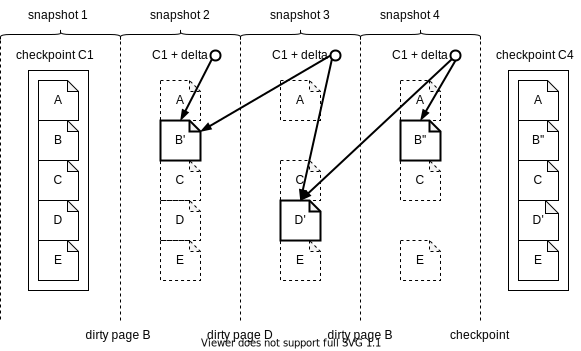
\includegraphics{/images/06-snapshot-deltas.svg}
\end{figure}

The runtime uses page maps in the following way:
\begin{enumerate}
  \item The system creates a "scratchpad" memory by constructing a patchwork from the checkpoint file and the running page deltas.
  \item The system executes a message on the actor state and detects the pages that the actor dirtied on the scratchpad.
  \item If the message execution succeeds, the system copies the contents of the dirty pages into the running delta.
  \item Otherwise, the system throws away the scratchpad.
\end{enumerate}

Once in a while, the system creates a new checkpoint by cloning the original checkpoint file and flushing dirty pages to the new file.
This procedure speeds up scratchpad construction and reduces memory pressure.

\section{detecting-memory-writes}{Detecting memory writes}

Detecting touched and dirtied memory pages is another challenging aspect of orthogonal persistence.
The system compiles actor's WebAssembly modules to native code.
How do you know which pages arbitrary code touched? 
There are multiple approaches to this problem:
\begin{itemize}
  \item 
    Compare the full memory before and after execution.
    This approach is easy to implement and works on all platforms, but it performs poorly on sizable memories and does not give us accessed pages.
  \item 
    Instrument the WebAssembly module before compiling it to native code.
    For example, we could add a system call before all \code{load} and \code{store} instructions to mark the corresponding pages as accessed or dirtied.
    This approach works on all platforms but can slow down execution by an order of magnitude.
  \item 
    Use memory protection and signal handlers to detect memory reads and writes at runtime.
    This approach works well on \textsc{unix} platforms and is reasonably efficient.
    We shall discuss this approach in more detail shortly.
  \item 
    Implement a custom filesystem backend as a \href{https://en.wikipedia.org/wiki/Filesystem_in_Userspace}{\textsc{fuse}} library, then \href{https://man7.org/linux/man-pages/man2/mmap.2.html}{memory-map} actor memory as a virtual file.
    The operating system will call into our library when the actor code reads from or writes to the memory-mapped file, allowing us to perform the required bookkeeping.
    This approach works great on platforms that support \textsc{fuse} (Linux and macOS), but it has some administrative disadvantages.
    For example, the replica will need priveledged access to be able to mount a virtual filesystem.
  \item 
    Use Linux \href{https://man7.org/linux/man-pages/man1/pmap.1.html}{pmap} utility to extract \href{https://techtalk.intersec.com/2013/07/memory-part-2-understanding-process-memory/#pmap-detailed-mapping}{memory access statistics} right after the message execution.
    This approach is very efficient, but it does not always produce deterministic results.
\end{itemize}

\subsection{signal-handler}{The signal handler}

The \href{https://man7.org/linux/man-pages/man2/mprotect.2.html}{memory protection \textsc{api}} allows us to set read and write permissions on page ranges.
If the process violates the permissions by reading a read-protected region or writing to a write-protected region, the operating system sends a signal (usually \code{SIGSEGV}) to the thread that triggered the violation.
The \href{https://man7.org/linux/man-pages/man7/signal.7.html}{signal handling \textsc{api}} allows us to intercept these signals and inspect the address that caused them.
We can build a robust and efficient memory access detection mechanism by combining these \textsc{api}s.

\begin{figure}
\marginnote{mn-mem-access-pseudocode}{Pseudocode of the memory access detection state machine.}
\begin{code}[rust]
let mut mem = construct_actor_memory();
let mut dirty_pages = bit_vector();
let mut touched_pages = bit_vector();

// Mark actor's memory as non-readable and non-writeabe.
\b{mprotect}(mem.start(), mem.len(), \b{PROT_NONE});

set_signal_handler(SIGSEGV, |address, is_read| {
  touched_pages.set(address.page_index());

  if is_read {
    // Allow the process to read from the page.
    // Subsequent read from the page will not trigger the
    // signal handler, but writes to the page will.
    mprotect(address.page_start(), PAGE_SIZE, \b{PROT_READ});
  } else {
    // Allow the process to read from and write to the page.
    // Subsequent reads from and writes to the page will not trigger
    // the signal handler.
    mprotect(address.page_start(), PAGE_SIZE, \b{PROT_READ} | \b{PROT_WRITE});
    dirty_pages.set(address.page_index());
  }
});

actor.execute_message(&mut mem, message);

// observe dirty_pages and touched_pages
\end{code}
\end{figure}

Let us see the state machine in action on a simple example:
an actor stores an array of integers; it needs to find a specific integer in the array and replace it with another.

\begin{figure}
\marginnote{mn-replace-func}{An example of a function triggering the memory access mechanism.}
\begin{code}[rust]
fn replace(array: &mut [u32], src: u32, dst: u32) {
  for i in 0..array.len() {
    if array[i] == src {
      array[i] = dst;
      break;
    }
  }
}
\end{code}
\end{figure}

To keep the example simple, let us assume that the array starts at page zero, and the integer to replace is at position \code{2000} in the array.
Before the execution begins, the entire memory has protection flags \code{PROT_NONE}.
As the actor executes the \code{replace} function, the following events occur:
\begin{enumerate}
  \item 
    The actor accesses \code{array\[0\]}.
    Since the corresponding memory page is read-protected, the load instruction generates a \code{SIGSEGV} signal.
    The system invokes the signal handler that marks the page as touched and sets the memory protection to \code{PROT_READ}.
    The context switches back to the actor code, which can now repeat the read operation successfully.
  \item 
    The actor accesses array elements \code{array\[1\]} through \code{array\[1023\]}\sidenote{sn-4096-1024}{A 4096-byte memory page can fit 1024 32-bit integers.} without interruption.
  \item 
    The actor accesses \code{array\[1024\]}.
    This element lives on the next page, which is still read-protected.
    The system behaves just as in step \circled{1}.
  \item 
    The actor accesses elements \code{array\[1025\]} through \code{array\[2000\]} without interruption.
  \item 
    The actor writes to \code{array\[2000\]}.
    The corresponding memory page is write-protected, so the store instruction generates a \code{SIGSEGV} signal.
    The context switches to the signal handler.
    The signal handler marks the page as dirty and removes the write protection by settings the protection flags to \code{PROT_READ | PROT_WRITE}.
    The actor code resumes and repeats the write, this time without interruption.
\end{enumerate}

\begin{figure}[grayscale-diagram]
\marginnote{mn-mm-states}{
  States of the memory mapping during \code{replace} function execution.
  Rectangles represent memory pages, hollow arrows---reads, solid arrows---writes.
}
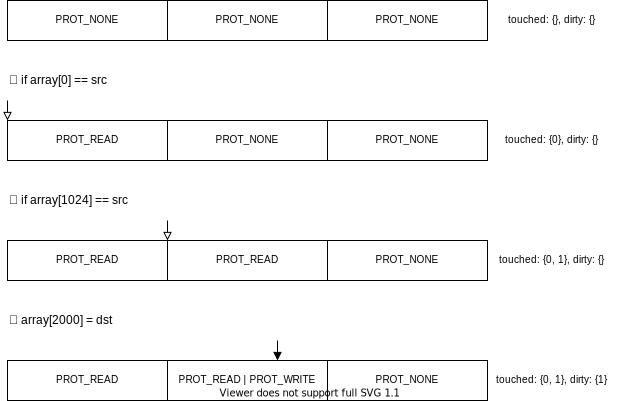
\includegraphics{/images/06-memory-mapping-states.svg}
\end{figure}

The signal handler approach is quite efficient in practice, and we can optimize it further:
\begin{itemize}
  \item 
    Instead of constructing the full actor memory in advance, we can populate it lazily when the actor first touches it.
    This optimization works best for fragmented memories with lots of page deltas.
  \item 
    Sequential memory access is a pervasive pattern worth optimizing.
    We can remove read protection from multiple consequent pages at once, removing the need to switch the execution context to the signal handler for each page.
    This optimization makes the mechanism less precise but can significantly improve execution speed.
  \item 
    We can speculatively remove write protection from multiple consequent pages to speed up sequential writes.
    We can later compare the contents of dirtied pages with the snapshot to validate our speculation.
\end{itemize}

\section{upgrades}{Surviving upgrades}

Orthogonal persistence creates an illusion that the program runs forever without interruption.
But what if we want to fix a bug in that program or add a new feature?
Can we do the upgrade without losing the program state?

At first sight, it might seem safe to swap the WebAssembly module of an actor without changing the contents of its memory.
Unfortunately, this seldom works in practice.

\begin{itemize}
  \item 
    The actor code expects a specific memory layout; changing data type definitions affects the layout.
    The new version of the code will not be able to make sense of the old memory.
  \item 
    The memory might contain pointers to functions.
    Changing the code might invalidate these pointers.
  \item 
    The code might have other expectations about the data besides the memory layout.
    For example, the new version of the code might use a different hash function for hash tables.
    Hash table lookups might start returning invalid results after the code swap.
\end{itemize}

The only known way to solve this issue is to rely on stable data representations.
There is a \href{https://github.com/WebAssembly/multi-memory}{proposal} that enables WebAssembly programs to access multiple disjoint memories.
\href{https://people.mpi-sws.org/~rossberg/}{Andreas Rossberg} suggested using the multi-memory feature to refine the persistence model with memory lifetimes.
For example, an actor could use the default memory (the memory with index zero) as mid-term storage that depends on the compiler's memory representation.
The actor could use other memories as long-term storage with a stable (ideally, language-independent) data layout.
The system would wipe out the transient memory during the upgrade but persist the long-term\sidenote{short-term-storage}{
  Andreas also proposed short-term memories with a lifetime of a single message execution.
  Such memories open up attractive optimization opportunities, but we did not have enough pressure to implement them. 
} storage. 

Since the IC needed to support upgrades before the multi-memory proposal was implemented, the runtime emulates one extra memory via the \href{https://smartcontracts.org/docs/interface-spec/index.html#system-api-stable-memory}{stable memory \textsc{api}}.
This \textsc{api} intentionally mimics WebAssembly \href{https://webassembly.github.io/bulk-memory-operations/core/exec/instructions.html#memory-instructions}{memory instructions} to facilitate future migration to multi-memory modules.
Internally, the main memory and the stable memory share the \href{#snapshots-deltas}{representation}.

Currently, most actors serialize their entire state to stable memory in the pre-upgrade hook and read it back in the post-upgrade hook.
There is an ongoing effort to build tools that make it easier to use stable memory as the primary data storage.

\section{conclusion}{Conclusion}

We examined the classical approach to orthogonal persistence and its \href{#actors}{synergy} with the actor model.
We learned about the \href{#snapshots-deltas}{page map}, the data structure that IC replicas use to store multiple versions of an actor's memory efficiently, and the \href{#signal-handler}{\textsc{sigsegv}-based memory access detection system}.
Lastly, we saw that orthogonal persistence is not the final solution to state persistence and why we need better tools to handle \href{#upgrades}{program upgrades}.

\section{references}{References}

The \href{https://github.com/dfinity/ic}{IC replica code} is open source.
In case you want to read the code that implements ideas from this article, here are a few pointers:
\begin{itemize}
  \item The \href{https://github.com/dfinity/ic/blob/3633026472367a413912bf797490c9336ba762f5/rs/execution_environment/src/hypervisor.rs#L1136}{function executing a single message}.
  \item The \href{https://github.com/dfinity/ic/blob/3633026472367a413912bf797490c9336ba762f5/rs/replicated_state/src/page_map.rs}{page map} module.
  \item The \href{https://github.com/dfinity/ic/blob/3633026472367a413912bf797490c9336ba762f5/rs/memory_tracker/src/lib.rs#L358}{naive} and the \href{https://github.com/dfinity/ic/blob/3633026472367a413912bf797490c9336ba762f5/rs/memory_tracker/src/lib.rs#L499}{optimized} signal handlers.
\end{itemize}
\end{document}

